\documentclass[12pt]{article}

\usepackage{blindtext}
\usepackage{alphabeta}
\usepackage[utf8]{inputenc}
\usepackage[main=greek, english]{babel}
\usepackage{hyperref}

\usepackage{titling}
\usepackage{graphicx}
\graphicspath{{images/}}

\begin{document}

\author{
    Μπίλιας Ευστάθιος
    \and
    Γκούντης Βασίλης
}

\title{Κλήσεις Συστήματος, Διαχείριση Διεργασιών και Διαδιεργασιακή
    Επικοινωνία}

\begin{titlepage}
    \begin{center}

        \Huge
        \textbf{Λειτουργικά Συστήματα Υπολογιστών}

        \vspace{0.5cm}
        \LARGE
        $1^η$ Εργαστηριακή Άσκηση

        \vspace{0.3cm}
        {\vspace{-2em}\let\newpage\relax\maketitle\vspace{-2em}}

        \vspace{0.8cm}

        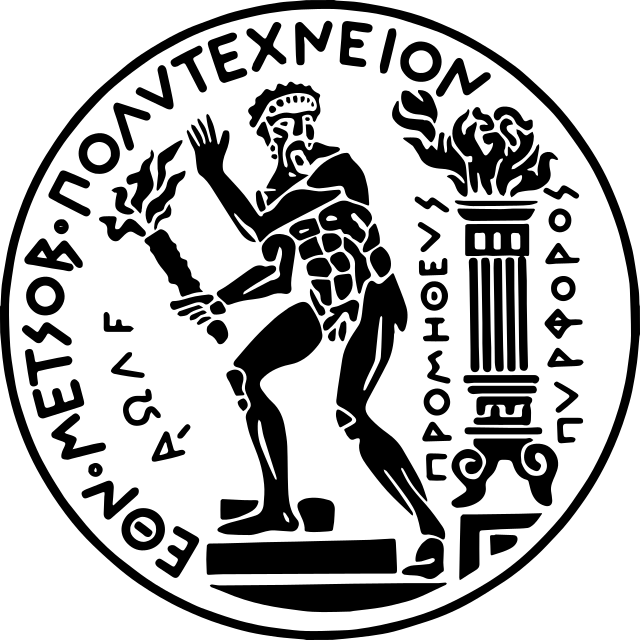
\includegraphics[width=0.3\textwidth]{logo.png}

        \vspace{0.8cm}
        \Large
        ΣΗΜΜΥ\\
        Εθνικό Μετσόβιο Πολυτεχνείο\\

    \end{center}
\end{titlepage}

\tableofcontents
\setcounter{page}{2}
\pagebreak

\section{Ανάγνωση και εγγραφή αρχείων στη \foreignlanguage{english}{C} \\ και
  με τη βοήθεια κλήσεων συστήματος}

Για την υλοποίηση της πρώτης άσκησης ξεκινήσαμε να διαβάζουμε τα
\foreignlanguage{english}{manuals} των εντολών που μας δοθήκαν
ως βοηθήματα.
Για την περαιτέρω κατανόηση τους, μελετήσαμε τις διαφάνειες και τα παραδείγματα
του μαθήματος και αφού
φτάσαμε σε σημείο να καταλαβαίνουμε πως λειτουργούν οι εντολές
\textbf{\foreignlanguage{english}{open, read, write}} και
\textbf{\foreignlanguage{english}{close}} ξεκινήσαμε να γράφουμε τον κώδικα μας
ακολουθώντας τα παραδείγματα.

\subsection{\foreignlanguage{english}{Open}}
Αρχικά, χρησιμοποιήσαμε την \textbf{\foreignlanguage{english}{open}} για να
ανοίξουμε τα αρχεία τα οποία μας δίνει ο χρήστης από τη
γραμμή εντολών και τις μεταβλητές \textbf{\foreignlanguage{english}{fpr}} και
\textbf{\foreignlanguage{english}{fpw}} στις οποίες αποθηκεύεται
η τιμή του \textbf{\foreignlanguage{english}{file descriptor}} που επιστρέφει η
\textbf{\foreignlanguage{english}{open}} ώστε να διαχωρίσουμε
το αρχείο ανάγνωσης από το αρχείο εγγραφής.

\subsection{\foreignlanguage{english}{Read}}
Στη συνέχεια,  κάνουμε την ανάγνωση του αρχείου μέσω της χρήσης της
\textbf{\foreignlanguage{english}{read}}, η οποία παίρνει σαν πρώτο
όρισμα το \textbf{\foreignlanguage{english}{fpr}}, που περιέχει τον
\textbf{\foreignlanguage{english}{file descriptor}} του αρχείου που θέλουμε να
διαβάσουμε, σαν δεύτερο όρισμα έναν \textbf{\foreignlanguage{english}{buffer}}
που έχουμε δηλώσει προηγουμένως και στον οποίο θα πραγματοποιηθεί
η ανάγνωση και σαν τρίτο όρισμα το μέγεθος που θέλουμε να διαβάσουμε, στην
περίπτωση μας θέλουμε να διαβάσουμε όσο χωράει ο
\textbf{\foreignlanguage{english}{buffer}}. Την
\textbf{\foreignlanguage{english}{read}} χρησιμοποιούμε μέσα σε ένα
\textbf{\foreignlanguage{english}{for loop}}
το οποίο τρέχει ασταμάτητα μέχρι να συναντήσει την
\textbf{\foreignlanguage{english}{break}}, την οποία συναντάει όταν ο τύπος
\textbf{\foreignlanguage{english}{rcnt}} γίνει 0 (μηδέν), δηλαδή όταν έχει
τελειώσει η ανάγνωση του αρχείου.
Μέσα στη \textbf{\foreignlanguage{english}{read}} υλοποιούμε επίσης και το
κομμάτι του κώδικα το οποίο ευθύνεται για την καταμέτρηση του χαρακτήρα
που έχουμε ζητήσει στη γραμμή εντολών. Για να επιτευχθεί αυτό, μεσα σε ένα
\textbf{\foreignlanguage{english}{for loop}} το οποίο εκτελείται από 0
μέχρι \textbf{\foreignlanguage{english}{rcnt}} δηλαδή μέχρι να διατρέξει όλα τα
στοιχειά του \textbf{\foreignlanguage{english}{buffer}} ελέγχεται αν η τιμή
στην θέση \textbf{\foreignlanguage{english}{i}} του πίνακα
\textbf{\foreignlanguage{english}{buff}} είναι ίση με τον χαρακτήρα
\textbf{\foreignlanguage{english}{sc}}
τον οποίο ψάχνουμε.
Κάθε φορά που θα εντοπίζεται ο χαρακτήρας θα ανεβαίνει και η μεταβλητή
\textbf{\foreignlanguage{english}{count}} την οποία έχουμε αρχικοποιήσει στο 0.

\subsection{\foreignlanguage{english}{Write}}
Παρακάτω, δημιουργούμε έναν άλλο πίνακα με το όνομα
\textbf{\foreignlanguage{english}{message}} στον οποίο τοποθετούμε το μήνυμα
που θέλουμε να
εμφανίζεται στο αρχείο εγγραφής. Και μέσα σε ένα
\textbf{\foreignlanguage{english}{while loop}} χρησιμοποιούμε την
\textbf{\foreignlanguage{english}{write}}
η οποία παίρνει σαν όρισμα το \textbf{\foreignlanguage{english}{file
        descriptor}} του αρχείου εγγραφής καθώς και το μήνυμα που εμφανίζεται
στον
πίνακα
\textbf{\foreignlanguage{english}{message}} ώστε να το γράψει μέσα στο αρχείο.
Επιπλέον, χρησιμοποιούμε τις \textbf{\foreignlanguage{english}{len}} και
\textbf{\foreignlanguage{english}{idx}} για να μας βοηθήσουν στην εγγραφή,
η \textbf{\foreignlanguage{english}{len}} περιέχει το μήκος του μηνύματος και η
\textbf{\foreignlanguage{english}{idx}} χρησιμοποιείται σαν κέρσορας
ώστε να γνωρίζουμε σε ποιο μέρος του μηνύματος βρισκόμαστε.

\subsection{\foreignlanguage{english}{Close}}
Τέλος, για να ολοκληρώσουμε χρησιμοποιούμε την
\textbf{\foreignlanguage{english}{close}} ώστε να κλείσουμε τα αρχεία που
είχαμε ανοίξει προηγουμένως.

\pagebreak

\section{Δημιουργία Διεργασιών}

\subsection{\foreignlanguage{english}{Greetings}}
Στο πρώτο ερώτημα της δεύτερης άσκησης το πρόγραμμα ξεκινά με μια κύρια
διεργασία (πατέρας) που δημιουργεί μια νέα διεργασία (παιδί) με την κλήση
\textbf{\foreignlanguage{english}{fork}}.

\subsubsection{Διεργασία Παιδί}
Αν η \textbf{\foreignlanguage{english}{fork}} επιστρέψει 0, βρισκόμαστε στη
διεργασία παιδιού, όπου καλούνται οι \textbf{\foreignlanguage{english}{getpid}}
και
\textbf{\foreignlanguage{english}{getppid}} για να πάρουν τα
\textbf{\foreignlanguage{english}{PID}} της διεργασίας παιδιού και του πατέρα
αντίστοιχα.
Στη συνέχεια, το παιδί καλεί τη συνάρτηση
\textbf{\foreignlanguage{english}{child}} για να τυπώσει ένα μήνυμα με αυτές
τις πληροφορίες.

\subsubsection{Διεργασία Πατέρας}
Αν η \textbf{\foreignlanguage{english}{fork}} επιστρέψει θετικό αριθμό,
βρισκόμαστε στη διεργασία πατέρα.
Ο πατέρας καλεί τη συνάρτηση \textbf{\foreignlanguage{english}{father}} με το
\textbf{\foreignlanguage{english}{PID}} της νέας διεργασίας (παιδιού)
και περιμένει το παιδί να τερματίσει με την κλήση
\textbf{\foreignlanguage{english}{wait}}. Μετά, ο πατέρας τυπώνει ένα μήνυμα
που δείχνει το αποτέλεσμα της αναμονής
χρησιμοποιώντας τη συνάρτηση
\textbf{\foreignlanguage{english}{explain\_wait\_status}}.

\subsubsection{\foreignlanguage{english}{Error}}
Αξίζει να σημειώθει οτάν η \foreignlanguage{english}{fork} επιστρέφει -1
αποτέλει σφαλμά.

\subsubsection{Βοηθητική συνάρτηση
    \foreignlanguage{english}{explain\_wait\_status}}
Την συνάρτηση \textbf{\foreignlanguage{english}{explain\_wait\_status}} την
πήραμε ετοιμή από τις διαφάνειες και την χρησιμοποιήσαμε για να παρατηρήσουμε
πως συμπεριφέρονται τα παιδιά διεργασίες.

\pagebreak

\subsection{Μεταβλητή $x$}
Αρχικά θέτουμε μια μεταβλητή $x=0$ στον πατέρα (\textbf{πρίν κάνουμε την
    \foreignlanguage{english}{fork}}).
Ύστερα μέσα στο παιδί αναθέτουμε την τιμή του $x$ σε 1, ενώ μέσα στον πατέρα
(αυτή τη φορά \textbf{μετά την \foreignlanguage{english}{fork}} και όταν αυτή
επιστρέφει θετικό αριθμό) την αναθέτουμε σε 2. Αυτό που παρατηρούμε είναι ότι
το παιδί
εκτυπώνει ότι $x=1$ και ο πατεράς ότι $x=2$.
Με λίγα λόγια συμπεραίνουμε ότι κανένας από τους δύο δεν εκτυπώνει $x=0$.

\subsection{Αναζήτηση χαρακτήρα από το παιδί}
Η φιλοσοφία του κωδικά είναι παρομοία με του κώδικα του πρώτου ερωτημάτος. Η
μόνη ουσιαστική
διαφορά είναι οτί τα \foreignlanguage{english}{read} και
\foreignlanguage{english}{write}, όπως και
η καταμέτρηση του χαρακτήρα θα γίνουν μόνο από το παιδί (δηλαδή μετά την
\foreignlanguage{english}{fork}
και οτάν αυτή επιστρέφει 0), ενώ ο πατέρας αναλαμβάνει αποκλειστικά τα
\foreignlanguage{english}{open} και
\foreignlanguage{english}{close} (μετά την \foreignlanguage{english}{fork},
αλλά αυτή την φορά οτάν επιστρέφει θετικό αριθμό).
Επίσης, χρησιμοποιούμε την \foreignlanguage{english}{wait} ώστε ο πατέρας να
περιμένει το παιδί να τερματίσει
πρίν κλείσει τα αρχεία.

\subsection{Χρήση \foreignlanguage{english}{execv} για εκτέλεση κώδικα από άλλο
    εκτελέσιμο}

Για την υλοποίηση του κώδικα αυτού του ερωτήματος ξεκινήσαμε διαβάζοντας το
\foreignlanguage{english}{manual} της \foreignlanguage{english}{exec} και
πιο συγκεκριμένα της \foreignlanguage{english}{execv}. Αφού καταλάβαμε πως
δουλεύει
η
\foreignlanguage{english}{execv} ξεκινήσαμε γράφοντας ότι χρειάζεται να
κληρονομήσει το παιδί πριν
καλέσουμε την \foreignlanguage{english}{fork}, τις μεταβλητές
\foreignlanguage{english}{pid\_t} για να
κρατήσει το \foreignlanguage{english}{PID} του παιδιού
και άλλες σχετικές πληροφορίες, μια μεταβλητή \foreignlanguage{english}{status}
που θα χρησιμοποιηθεί για
να αποθηκεύσει την κατάσταση της αναμονής και ένα πίνακα χαρακτήρων
\foreignlanguage{english}{args} που
περιέχει τα επιχειρήματα για το πρόγραμμα που θα εκτελεστεί από την διεργασία
παιδί. Το πρώτο στοιχείο είναι το μονοπάτι
προς το εκτελέσιμο του προγράμματος και τα υπόλοιπα είναι τα επιχειρήματα που
λαμβάνει το \foreignlanguage{english}{argv} από τη
γραμμή εντολών τα οποία είναι αναγκαία για να λειτουργήσει το πρόγραμμα που
θέλουμε να εκτελέσουμε. Αφού γίνει η
\foreignlanguage{english}{fork} και επιστραφεί η τιμή 0 δηλαδή ότι βρισκόμαστε
στην διεργασία παιδί
καλείται η \foreignlanguage{english}{execv} με τα επιχειρήματα
που είχαν οριστεί νωρίτερα για να εκτελέσει το πρόγραμμα
\foreignlanguage{english}{./a1.1} με τα δεδομένα
από τα \foreignlanguage{english}{argv[1], argv[2], argv[3]}.

\pagebreak

\section{Διαδιεργασιακή Επικοινωνία}
Ο κώδικας αυτού του ερωτήματος είναι παρόμοιος με αυτόν του ερωτήματος 2 δηλαδή
το άνοιγμα και κλείσιμο των αρχείων γίνεται στον πατερά με μια διαφορά πως σε
αυτή την περίπτωση το γράψιμο στο αρχείο εγγραφής γίνεται επίσης από τον
πατερά. Έχουμε προσθέσει μια \foreignlanguage{english}{global} μεταβλητή $n$
στην αρχή του κώδικα, η οποία
ορίζει πόσες διεργασίες θα δημιουργηθούν. Χρησιμοποιούμε την εντολή
\foreignlanguage{english}{signal} για
να εντοπίσουμε το σήμα \foreignlanguage{english}{SIGINT} που θέλουμε και όταν
το κάνουμε αυτό καλούμε την
συνάρτηση \foreignlanguage{english}{handler} που έχουμε ορίσει στην αρχή του
κώδικα η οποία διαχειρίζεται
το σήμα, στην περίπτωση μας θα τυπώνει την σταθερά $n$ η οποία εκφράζει τον
αριθμό των διεργασιών οι οποίες αναζητούν τον χαρακτήρα. Μέσα σε ένα βρόγχο ο
οποίος επαναλαμβάνεται $n$ φορές δημιουργούμε ένα
\foreignlanguage{english}{pipe} και κάνουμε \foreignlanguage{english}{fork} την
γονική διεργασία, με αυτό τον τρόπο εξασφαλίζουμε ότι κάθε διεργασία παιδί που
θα δημιουργείτε θα έχει και το δικό του \foreignlanguage{english}{pipe}. Έπειτα, κλείνουμε το \foreignlanguage{english}{read end} του
\foreignlanguage{english}{pipe} της διεργασίας παιδί, διότι το παιδί θέλουμε να γραφεί μόνο. Και
ξαναχρησιμοποιούμε την εντολή \foreignlanguage{english}{signal} αυτή τη φορά όχι για να διαχειριστούμε το
σήμα που ψάχνουμε αλλά για να το αγνοήσουμε με τη χρήση του \foreignlanguage{english}{SIG\_IGN}. Στη
συνέχεια εκτελούμε τη \foreignlanguage{english}{read}, γράφουμε το αποτέλεσμα του \foreignlanguage{english}{counter} στο \foreignlanguage{english}{pipe} και
βάζουμε το παιδί να κοιμηθεί για 1 δευτερόλεπτο ώστε να έχουμε χρόνο κατά την
εκτέλεση να στείλουμε το σήμα \foreignlanguage{english}{SIGINT}. Τέλος, κλείνουμε το \foreignlanguage{english}{write end} του \foreignlanguage{english}{pipe}
από την πλευρά του πατερά, καλούμε την \foreignlanguage{english}{explain\_wait\_status} για να μας
εξηγήσει
πως εκτελέστηκαν τα παιδιά και πηγαίνουμε και διαβαζουμε από το \foreignlanguage{english}{pipe} το
αποτέλεσμα που μας έστειλε το παιδί. Αυτό το κάνουμε μέσα σε ένα βρόγχο ο
οποίος θα τρέξει $n$ φορές δηλαδή για όλα τα παιδιά και στο τέλος χρησιμοποιούμε
το \foreignlanguage{english}{count} για να αθροίσουμε όλα τα \foreignlanguage{english}{counters} δηλαδή τα αποτελέσματα όλων των
παιδιών. Αφού το κάνουμε αυτό πηγαίνουμε και γράφουμε στο αρχείο εγγραφής το
\foreignlanguage{english}{count} και κλείνουμε τα ανοιχτά αρχεία.

\end{document}